\documentclass{article}
\usepackage[utf8]{inputenc}
\usepackage{amsmath, amssymb}
\usepackage{setspace}
\usepackage{tikz}

\onehalfspacing

\title{Problem Set 12: Graphs, Networks, Incidence Matrices}
\author{Tiago C. Botelho}
\date{\today}

\begin{document}

\maketitle

\noindent \textbf{Problem 12.1:} First thing we'll do is write the incidence matrix for the square graph presented. Recall that each row represents an edge, and each column represents a node. We have:

\[
A = \begin{bmatrix}
-1 & \phantom{-}1 & \phantom{-}0 & \phantom{-}0\\
\phantom{-}0 & -1 & \phantom{-}1 & \phantom{-}0\\
\phantom{-}0 & \phantom{-}0 & \phantom{-}1 & -1\\
-1 & \phantom{-}0 & \phantom{-}0 & \phantom{-}1\\
\end{bmatrix}.
\]

We could solve $A\mathbf{x = 0}$, but really all it takes is some simple physical intuition: vectors in the nullspace have uniform potential, \textit{i.e.}, a basis for the nullspace is the vector

\[
\mathbf{1} = \begin{bmatrix}
1\\
1\\
1\\
1\\
\end{bmatrix},
\]

so the nullspace $\mathcal{N}(A)$ is the set of multiples of $\mathbf{1}$.

We know that $(1, 0, 0, 0)$ is \textit{not} in the row space of $A$ because of Kirchhoff's law! Current does not accumulate at any of the nodes -- what comes in must go out -- so we can't have one unit of current at a node (in particular, at the first node) that doesn't flow somewhere else.

\noindent \textbf{Problem 12.2:} There's no point in carrying out this computation without the aid of computers, especially these days; with the aid of \texttt{numpy}, we find that:

\[
A^{T}CA = \begin{bmatrix}
\phantom{-}2 & -1 & \phantom{-}0 & -1\\
-1 & \phantom{-}3 & -2 & \phantom{-}0\\
\phantom{-}0 & -2 & \phantom{-}4 & -2\\
-1 & \phantom{-}0 & -2 & \phantom{-}3\\
\end{bmatrix}.
\]

The row reduced form is:

\[
R^{*} = \begin{bmatrix}
1 & 0 & 0 & -1\\
0 & 1 & 0 & -1\\
0 & 0 & 1 & -1\\
0 & 0 & 0 & \phantom{-}0\\
\end{bmatrix}
\]

and the vector of dependent variables becomes:

\[
\mathbf{f}_R = \begin{bmatrix}
\phantom{-}0.5\\
\phantom{-}0\\
-0.25\\
\phantom{-}0
\end{bmatrix}.
\]

So a solution is $\mathbf{x} = (0.5,0.0,-0.25,0.0)$. We can check this using \texttt{numpy}, and indeed it works. We find $\mathbf{y} = (0.5, 0.5, 0.5, 0.5)$.

\begin{center}
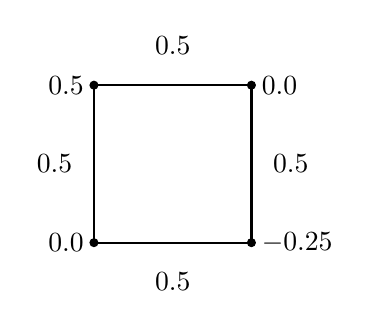
\begin{tikzpicture}
    \draw [fill] (0, 0) circle [radius=.05];
    \draw [fill] (0, 2) circle [radius=.05];
    \draw [fill] (2, 0) circle [radius=.05];
    \draw [fill] (2, 2) circle [radius=.05];
    \draw[thick] (0, 0) node[left] {$0.0$} -- (0, 2) node[left] {$0.5$} -- (2, 2) node[right] {$0.0$} -- (2, 0) node[right] {$-0.25$} -- (0, 0);
    \node at (-0.5, 1) {$0.5$};
    \node at (2.5, 1) {$0.5$};
    \node at (1, -0.5) {$0.5$};
    \node at (1, 2.5) {$0.5$};
\end{tikzpicture}
\end{center}

\end{document}